\documentclass[11pt, twoside, pdftex]{article}


% This includes all the settings that we should use for the document
\newcommand{\PDFTitle}{Using Terminals}
\newcommand{\commonPath}{../../Common}
\newcommand{\datePublished}{Mar 2022}

\newcommand{\versnum}{21.1} %version number quartus/AMP
\newcommand{\quartusname}{Quartus\textsuperscript{\textregistered} Prime}	
\newcommand{\textBar}{For \quartusname{} \versnum{}}
\newcommand{\thisyear}{2022 } %for copyright
\newcommand{\company}{FPGAcademy.org}
\newcommand{\longteamname}{FPGAcademy.org}
\newcommand{\teamname}{FPGAcademy}
\newcommand{\website}{FPGAcademy.org}

\newcommand{\productAcronym}{AMP}
\newcommand{\productNameShort}{Monitor Program}

\newcommand{\productNameMedTM}{Monitor Program}
\newcommand{\productNameMed}{Monitor Program}

%\newcommand{\headerLogoFilePath}[1]{#1/FPGAcademy.png}



\setlength\topmargin{-0.25in}
\setlength\headheight{0in}
\setlength\headsep{0.35in}
\setlength\textheight{8.5in}
\setlength\textwidth{7in}
\setlength\oddsidemargin{-0.25in}
\setlength\evensidemargin{-0.25in}
\setlength\parindent{0.25in}
\setlength\parskip{0in} 

\pdfpagewidth 8.5in
\pdfpageheight 11in

% listings is a package that supports encapsulating source code in LaTeX conveniently

\usepackage{listings}
% add support for graphics
\usepackage{graphicx}
\usepackage[usenames, dvipsnames]{color}

\def\expandparam\lstinputlisting[#1]#2{\edef\tmp{\noexpand\lstinputlisting[#1]{#2}}\tmp}

\widowpenalty 10000
\clubpenalty 10000

%%%%%%%%%%%%%%%%%%%% Source Code Formatting %%%%%%%%%%%%%%%%%%%%
\definecolor{globalCommentColour}{rgb}{0.588,0.588,0.588}

%%%%%%%%%%%%%%%%%%%%%%%%%%%%%%%%%%%%%%%%%%%%%%%%%%%%
% Defining a NiosII ASM highlighter for lstlisting
\lstdefinelanguage[NiosII]{Assembler} {
 	morekeywords={add, addi, and, andhi, andi, beq, bge, bgeu, bgt, bgtu, ble,  bleu, blt, bltu, bne, br, break,% 
 	bret, call, callr, cmpeq, cmpeqi, cmpge, cmpgei, cmpgeu, cmpgeui, cmpgt, cmpgti, cmpgtu, cmpgtui, cmple,%
 	cmplei, cmpleu, cmpleui, cmplt, cmplti, cmpltu, cmpltui, cmpne, cmpnei, custom, div, divu, eret, flushd,%
 	flushda, flushi, flushp, initd, initda, initi, jmp, jmpi, ldb, ldbio, ldbu, ldbuio, ldh, ldhio, ldhu, ldhuio,%
 	ldw, ldwio, mov, movhi, movi, movia, movui, mul, muli, mulxss, mulxsu, mulxuu, nextpc, nop, nor, or, orhi, ori,%
 	rdctl, rdprs, ret, rol, roli, ror, sll, slli, sra, srai, srl, srli, stb, stbio, sth, sthio, stw, stwio,%
 	sub, subi, sync, trap, wrctl, wrtcl, wrprs, xor, xori, xorhi, xori},% 	
 	morekeywords=[2]{.abort, .ABORT, .align, .app-file, .ascii, .asciz, .balign, .byte, .comm, .data, .def,%
 	.desc, .dim, .double, .eject, .else, .end, .endef, .endif, .equ, .equiv, .err, .extern, .file, .fill, .float,%
 	.global, .globl, .hword, .ident, .if, .include, .int, .irp, .irpc, .lcomm, .lflags, .line, .linkonce, .ln,%
 	.list, .long, .macro, .mri, .nolist, .octa, .org, .p2align, .psize, .quad, .rept, .sbttl, .scl, .section,%
 	.set, .short, .single, .size, .sleb128, .skip, .space, .stadb, .stabn, .stabs, .string, .symver, .tag,%
 	.text, .title, .type, .val, .uleb128, .word},% 	
 	morekeywords=[3]{et, bt, gp, sp, fp, ea, sstatus, ra, pc, status, estatus, bstatus, ienable, ipending, cpuid,%
 	exception, pteaddr, tlbacc, tlbmisc, eccinj, badaddr, config, mpubase, mpuacc},% 	
 	sensitive=t,%
 	alsoletter=.,%
	morestring=[b]",%
 	morecomment=[s]{/*}{*/},%
 	morecomment=[l]\#,%
   }[keywords,comments,strings]
   
   %% NOTE: morekeywords=[2] are GNU directives.
   
   \definecolor{niosInstructionColour}{rgb}{0.000,0.608,0.000}
   \definecolor{niosDirectiveColour}{rgb}{0.000,0.000,0.902}
   \definecolor{niosSpecialRegColour}{rgb}{0.000,0.000,0.000}
   \definecolor{niosStringColour}{rgb}{0.808,0.482,0.000}
   
   %% NOTE: To make bold use: =\bfseries\color{<colour>}
   \lstdefinestyle{defaultNiosStyle} {
   language=[NiosII]{Assembler},
   stringstyle=\color{niosStringColour},
   keywordstyle=\color{niosInstructionColour},
   keywordstyle=[2]\color{niosDirectiveColour},
   keywordstyle=[3]\itshape\color{niosSpecialRegColour}
   }
%%%%%%%%%%%%%%%%%%%%%%%%%%%%%%%%%%%%%%%%%%%%%%%%%%%%

%%%%%%%%%%%%%%%%%%%%%%%%%%%%%%%%%%%%%%%%%%%%%%%%%%%%
% Defining a ArmA9 ASM highlighter for lstlisting
\lstdefinelanguage[ArmA9]{Assembler} {
 	morekeywords={ADC, ADD, ADDS, AND, ANDS, B, BAL, BEQ, BGE, BGT, BL, BLT, BIC, BKPT, BLX, BNE, BX, CDP, CLZ, CMN, CMP, EOR,%
 	EORS, LDC, LDM, LDR, LDRB, LDRBT, LDRH, LDRSB, LDRSH, LDRT, LSL, MCR, MLA, MOV, MOVW, MOVT, MRC, MRS, MSR, MUL, MVN, ORR, PLD,%
 	ROR, RSB, RSC, SBC, SMLAL, SMULL, STC, STM, STR, STRB, STRBT, STRH, STRT, SUB, SUBS, SWI, SWP, SWPB, TEQ, UMLAL,
 	PUSH, POP, MOVS, RORS, LSR},%
 	morekeywords=[2]{.abort, .ABORT, .align, .app-file, .ascii, .asciz, .balign, .byte, .comm, .data, .def,%
 	.desc, .dim, .double, .eject, .else, .end, .endef, .endif, .equ, .equiv, .err, .extern, .file, .fill, .float,%
 	.global, .globl, .hword, .ident, .if, .include, .int, .irp, .irpc, .lcomm, .lflags, .line, .linkonce, .ln,%
 	.list, .long, .macro, .mri, .nolist, .octa, .org, .p2align, .psize, .quad, .rept, .sbttl, .scl, .section,%
 	.set, .short, .single, .size, .sleb128, .skip, .space, .stadb, .stabn, .stabs, .string, .symver, .tag,%
 	.text, .title, .type, .val, .vectors, .uleb128, .word},%
 	morekeywords=[3]{SP, PC, MIDR, CTR, TCMTR, TLBTR, MPIDR, ID_PFR0, ID_PFR1, ID_DFR0, ID_MMFR0, ID_MMFR1, ID_MMFR2,%
 	ID_MMFR3, ID_ISAR0, ID_ISAR1, ID_ISAR2, ID_ISAR3, ID_ISAR4, CCSIDR, CLIDR, AIDR, CSSELR, TTBR0, TTRB1, TTBR2, DACR,%
 	DFSR, IFSR, ADFSR, AIFSR, DFAAR, IFAR, ICIALLUIS, BPIALLIS, PAR, ICIALLU, ICIMVAU, BPIALL, DCIMVAC, DCISW, V2PCWPR,%
 	DCCVAC, DCCSW, DDIMVAC, DCISW, TLBALLIS, TLBIMVAIS, TLBIASIDIS, TLBIMVAAIS, TLBIALL, TLBIMVA, TLBIASID, TLBIMVAA,%
 	PMCR, PMCNTENSET, PMCNTENCLR, PMOVSR, PMSWINC, PMSELR, PMXEVTYPER, PMXEVCNTR, PMUSERENR, PMINTENSET, PMINTENCLR,%
 	PRRR, NRRR, PLEIDR, PLEASR, PLEFSR, PLEUAR, PLEPCR, VBAR, MVBAR, ISR, FCSEIDR, CONTEXTIDR, TPIDRURW, TPIDRURO, TPIDRPRW},%
 	sensitive=f,%
 	alsoletter=.,%
	morestring=[b]",%
 	morecomment=[s]{/*}{*/},%
 	morecomment=[l]{//},%
   }[keywords,comments,strings]
   
   %% NOTE: morekeywords=[2] are GNU directives.
   
   \definecolor{armInstructionColour}{rgb}{0.000,0.608,0.000}
   \definecolor{armDirectiveColour}{rgb}{0.000,0.000,0.902}
   \definecolor{armSpecialRegColour}{rgb}{0.000,0.000,0.000}
   \definecolor{armStringColour}{rgb}{0.808,0.482,0.000}
   
   \lstdefinestyle{defaultArmStyle} {
   language=[ArmA9]{Assembler},
   stringstyle=\color{armStringColour},
   keywordstyle=\color{armInstructionColour},
   keywordstyle=[2]\color{armDirectiveColour},
   keywordstyle=[3]\itshape\color{armSpecialRegColour}
   }
%%%%%%%%%%%%%%%%%%%%%%%%%%%%%%%%%%%%%%%%%%%%%%%%%%%%

%%%%%%%%%%%%%%%%%%%%%%%%%%%%%%%%%%%%%%%%%%%%%%%%%%%%
% Defining style for the verilog.

\definecolor{verilogCommentColour}{rgb}{0.000,0.502,0.000}

\lstdefinestyle{defaultVerilogStyle} {
language={Verilog},
keywordstyle=\color{blue},
commentstyle=\color{verilogCommentColour}
}
%%%%%%%%%%%%%%%%%%%%%%%%%%%%%%%%%%%%%%%%%%%%%%%%%%%%

%%%%%%%%%%%%%%%%%%%%%%%%%%%%%%%%%%%%%%%%%%%%%%%%%%%%
% Defining style for the vhdl.
\lstdefinestyle{defaultVHDLStyle} {
language={VHDL},
keywordstyle=\color{blue},
commentstyle=\color{verilogCommentColour}
}
%%%%%%%%%%%%%%%%%%%%%%%%%%%%%%%%%%%%%%%%%%%%%%%%%%%%

%%%%%%%%%%%%%%%%%%%%%%%%%%%%%%%%%%%%%%%%%%%%%%%%%%%%
% Java
\definecolor{javaStringColour}{rgb}{0.808,0.482,0}
%%%%%%%%%%%%%%%%%%%%%%%%%%%%%%%%%%%%%%%%%%%%%%%%%%%%

%%%%%%%%%%%%%%%%%%%%%%%%%%%%%%%%%%%%%%%%%%%%%%%%%%%%
% Defining language styles
% C
\definecolor{CStringColour}{rgb}{0.808,0.482,0}
%%%%%%%%%%%%%%%%%%%%%%%%%%%%%%%%%%%%%%%%%%%%%%%%%%%%

%%%%%%%%%%%%%%%%%%%%%%%%%%%%%%%%%%%%%%%%%%%%%%%%%%%%
% Defining extended LaTeX language.
\lstdefinelanguage[LocalLaTeX]{TeX}[LaTeX]{TeX}%
 	{moretexcs={bf, it, sf, lstset},%
   	}%

\lstdefinestyle{defaultLocalLatexStyle} {
language=[LocalLatex]{TeX},
keywordstyle=\color{blue}\bfseries,
keywordstyle=[2]\color{blue},
keywordstyle=[3]\color{blue}\bfseries
}
%%%%%%%%%%%%%%%%%%%%%%%%%%%%%%%%%%%%%%%%%%%%%%%%%%%%

\lstset{
%language = C,
%language = Verilog,
%basicstyle=\color{black}\rmfamily\ttfamily,
basicstyle=\small\color{black}\ttfamily,
commentstyle=\small\color{globalCommentColour}\itshape\ttfamily,
keywordstyle=\small\color{blue}\bfseries\ttfamily,
showstringspaces=false,
frame=none, %lines % boxed listings
breaklines=true,
breakatwhitespace=true,
tabsize=4
}
%%%%%%%%%%%%%%%%%%%%%%%%%%%%%%%%%%%%%%%%%%%%%%%%%%%%%%%%%%%%%%%%


%\usepackage[centering]{geometry}.
%%%%%%%%%%%%%%%%%%%%%%%%%%%%%%%%%%%%%%%%%%%%%%%%%%%
% Document Settings
\usepackage[labelsep=period]{caption}
% we can choose a better font later
%\usepackage{palatino}
\usepackage{fourier}
%\fontencoding{T1}
% include common used symbols
\usepackage{textcomp}
% add support for graphics
\usepackage{graphicx}
\usepackage[usenames, dvipsnames]{color}
% enable to draw thick or thin table hlines
\setlength{\doublerulesep}{\arrayrulewidth}
\usepackage{longtable}
\setlongtables
%\usepackage{array}
% It may be better to use PDFLaTeX as it can generate bookmarks for the
% document

% Add some useful packages
\usepackage{ae,aecompl}
\usepackage{epsfig,float,times}

% reset the font for section
\usepackage{sectsty}
%\allsectionsfont{\fontfamily{ptm}\selectfont}
\allsectionsfont{\usefont{OT1}{phv}{bc}{n}\selectfont}

% use compact space for sections
\usepackage[compact]{titlesec}
\titlespacing{\section}{0pt}{0.2in}{*0}
\titlespacing{\subsection}{0pt}{0.1in}{*0}
\titlespacing{\subsubsection}{0pt}{0.05in}{*0}

% fancyhdr header and footer customization
\usepackage{layout}
\usepackage{fancyhdr}
\pagestyle{fancy}
\fancyhead{}
\fancyhead[R]{\textit{\tiny{\textBar}}}
\fancyfoot{}
\fancyfoot[LO,
RE]{\textrm{\href{https://www.fpgacademy.org}{\small \longteamname}} \\ {\small \datePublished }}
\fancyfoot[RO, LE]{\small \thepage}
% two-side settings
%\fancyhead{} % clear all header fields
%\fancyfoot{} % clear all footer fields
%\fancyfoot[LE,RO]{\thepage}
\renewcommand{\headrulewidth}{2pt}
\renewcommand{\headrule}{{\color{blue} \hrule width\headwidth height\headrulewidth \vskip-\headrulewidth}}
\renewcommand{\footrulewidth}{0pt}

% Format the footer on page 1
\fancypagestyle{plain}{
\fancyhead{}
\fancyfoot{}
\fancyfoot[LO,
RE]{\textrm{\href{https://www.fpgacademy.org}{\small \longteamname}} \\ {\small \datePublished }}
\fancyfoot[RO, LE]{\small \thepage}
\renewcommand{\headrulewidth}{0pt}
}
% adjust some setting to try to make the figure stay in the same page with text
% Reference: 	http://www.cs.uu.nl/~piet/floats/node1.html
%   			http://mintaka.sdsu.edu/GF/bibliog/latex/floats.html
%   General parameters, for ALL pages:
\renewcommand{\topfraction}{0.9}	% max fraction of floats at top
\renewcommand{\bottomfraction}{0.8}	% max fraction of floats at bottom
%   Parameters for TEXT pages (not float pages):
\setcounter{topnumber}{3}
\setcounter{bottomnumber}{3}
\setcounter{totalnumber}{5}     % 2 may work better
\setcounter{dbltopnumber}{2}    % for 2-column pages
\renewcommand{\dbltopfraction}{0.9}	% fit big float above 2-col. text
\renewcommand{\textfraction}{0.07}	% allow minimal text w. figs
%   Parameters for FLOAT pages (not text pages):
\renewcommand{\floatpagefraction}{0.7}	% require fuller float pages
% N.B.: floatpagefraction MUST be less than topfraction !!
\renewcommand{\dblfloatpagefraction}{0.7}	% require fuller float pages
%%%%%%%%%%%%%%%%%%%%%%%%%%%%%%%%%%%%%%%%%%%%%%%%%%%
% remember to use [htp] or [htpb] for placement
%%%%%%%%%%%%%%%%%%%%%%%%%%%%%%%%%%%%%%%%%%%%%%%%%%%

% set no indent for paragraph
\setlength{\parindent}{0em}
\addtolength{\parskip}{11pt}
\newcommand{\compact}{[topsep=0pt]}
% use this package to reduce space
\usepackage{enumitem}
\usepackage{multirow}
\usepackage{rotating}
\usepackage{pifont}
\usepackage{dingbat}
\newcommand{\itemsecond}{$\circ$}
%
%%%%%%%%%%%%%%%%%%
\date{}
\author{}
%%%%%%%%%%%%%%%%%%
\newcommand{\de}{DE-series}
\newcommand{\up}{FPGAcademy}
\newcommand{\fabric}{Avalon Switch Fabric}
\newcommand{\TODO}[1]{\textcolor{red}{\textbf{TODO}: #1}}
\def\registered{{\ooalign{\hfil\raise .00ex\hbox{\scriptsize R}\hfil\crcr\mathhexbox20D}}}

% enable url and reference(bookmarks) in pdf
\usepackage{url}
\usepackage[pdftex, colorlinks]{hyperref}
\hypersetup{%
pdftitle={\PDFTitle},
linkcolor=blue,
hyperindex=true,
pdfauthor={\longteamname},
pdfkeywords={FPGAcademy, Academic Program, Example System},
bookmarksnumbered,
bookmarksopen=false,
filecolor=blue,
pdfstartview={FitH},
urlcolor=blue,
plainpages=false,
pdfpagelabels=true,
linkbordercolor={1 1 1} %no color for link border
}%
%%%%%%%%%%%%%%%%%%%%%%%%%%%%%%%%%%%%%%%%%%%%%%%%%%%
\setlength{\fboxsep}{0.7pt}
\setlength{\fboxrule}{0.5pt}

\newcommand{\red}[1]{{\color{red}\sf{#1}}}
\newcommand{\blue}[1]{{\color{blue}\sf{#1}}}



%%%%%%%%%%%%%%%%%%%%%%%%%
% Add title
\newcommand{\doctitle}{Using Terminals with \\ DE-Series Boards }
\newcommand{\dochead}{Using Terminals with DE-Series Boards}
% Usually no need to change these two lines
\title{\fontfamily{phv}\selectfont{\doctitle} }
\chead{ \small{\textsc{\bfseries \dochead} } }
% Customizations
%%%%%%%%%%%%%%%%%%%%%%%%%
% Allows multiple figures per page

\renewcommand\floatpagefraction{.9}
\renewcommand\topfraction{.9}
\renewcommand\bottomfraction{.9}
\renewcommand\textfraction{.1}   
\setcounter{totalnumber}{50}
\setcounter{topnumber}{50}
\setcounter{bottomnumber}{50}
\raggedbottom

%%%%%%%%%%%%%%%%%%
%%% DOCUMENT START
%\begin{document}
\begin{document}
\begin{table}
    \centering
    \begin{tabular}{p{5cm}p{4cm}}
        \hspace{-3cm}
        &
        \raisebox{1\height}{\parbox[h]{0.5\textwidth}{\Large\fontfamily{phv}\selectfont{\textsf{\doctitle}}}}
    \end{tabular}
    \label{tab:logo}
\end{table}

\colorbox[rgb]{0,0.384,0.816}{\parbox[h]{\textwidth}{\color{white}\textsf{\textit{\textBar}}}}

\thispagestyle{plain}
 
\section{Introduction}

This tutorial provides an introduction to using terminals to communicate with programs compiled for Nios\textsuperscript{\textregistered} II and ARM* processors on the Intel\textsuperscript{\textregistered} DE-series FPGA boards. The tutorial demonstrates how to write C and assembly code for these processors to send and receive characters to and from a host PC. On the host PC side, the tutorial describes how to use the \productNameMed{}'s terminal window, as well as third-party terminal programs such as Putty, to send and receive characters to and from the FPGA board.

The reader is expected to have a basic understanding of C and assembly languages, and to be familiar with the \productNameMed{} software.

{\bf Contents}:
\begin{itemize}
\item Introduction to terminals
\item Using the JTAG* UART terminal
\item Using the RS232 UART terminal
\item Using the USB UART terminal
\item Using the ARM Semihosting terminal
%\item Using the Altera Monitor Program's Terminal Window
\end{itemize}
\clearpage
\newpage

\section{Background}

%A terminal is a program that receives and displays text data from another program to the user, and allows the user to input text data into that other program.
%A terminal is a program that allows a user to read text data from and enter text data to another program. 
A terminal is a program that receives and displays text data; it also allows a user to input text data for transmission to other programs.
Most programmers will be familiar with the Linux* console (a kind of terminal), where a program can call the printf and scanf functions to display text to, and read text from, the terminal. In this case, the program and the terminal both run on the same system, and the communication between the two is facilitated by the Linux operating system. 

%Sometimes, a user would like to use a terminal to communicate with a remote program. Here, we define remote program as one that is running on a system that is not the one on which the terminal is running. 
%There are situations where the program to which a user would like to communicate is running on a separate device or system than the one on which the user's terminal is running. 
%In this case, there needs to be some communication link between the two systems, to facilitate sending characters between them. Figure ASDF shows a high level diagram of this arrangement. 

%When developing a program for a Nios II or ARM processor running on an FPGA board, it is often convenient to use a terminal on the host PC to communicate with the remote program running on the board. To accomplish this, the terminal and the remote program can use one of the various possible communication links between the PC and the FPGA board. This tutorial discusses the use of the following communication links: JTAG UART, RS232 UART, USB UART, and Semihosting.

Sometimes, it is necessary to use a terminal to communicate with a remote program - one that is running on a different system than the terminal. For example, when developing a program for a Nios II or ARM processor running on an Intel FPGA board, it is convenient to use a terminal on the host PC to communicate with the program running on the board. Because the terminal and the remote program run on separate systems, some sort of communication link between the two systems is required for data transmission. The DE-series FPGA boards provide a number of ways to establish a communication link with the host PC: JTAG UART, RS232 UART, USB UART, and Semihosting. This tutorial describes how to write remote program code for Nios II and ARM processors to send and receive characters through these communication links. As well, it describes how to launch a terminal on the host PC to connect to these links.

%Sometimes, it is necessary to use a terminal to communicate with a remote program - one that is running on a different
%system than the terminal. For example, when developing a program for a Nios II or ARM processor running on an
%FPGA board, it is convenient to use a terminal on the host PC to communicate with the program running on the
%board. To accomplish this, some sort of communication link must be established between the host PC and the FPGA
%board. Then, the program running on the board can send and receive characters through this link to and from a
%terminal on the host PC. This tutorial discusses the use of the following communication links available for use with
%the DE-series boards: JTAG UART, RS232 UART, USB UART, and Semihosting.

%\section{Design Example}



\section{Using Terminals}

This section describes the use of the JTAG UART, RS232 UART, USB UART, and Semihosting terminals. Because each terminal type requires a particular communication link, some boards may not support certain terminals. For example, the RS232 UART terminal uses a RS232 serial cable to transmit characters. Only the DE0 and DE2-115 boards contain RS232 ports and therefore support this terminal type. Table 1 provides a full list of the terminals supported by each DE-series board. 

\begin{table}[h]

    \centering
    \begin{tabular}{|c|c|c|c|c|}
        \hline
        \multicolumn{5}{|l|}{\textit{\textbf{Table 1. Supported Terminals by Board}}}
        \\\hline
            \textbf{}
            & \textbf{JTAG UART}
            & \textbf{RS232 UART}
            & \textbf{USB UART}
            & \textbf{Semihosting}
        \\\hline
            DE0-CV
            & Yes
            & 
            & 
            & 
        \\\hline
            DE0-Nano
            & Yes
            & 
            & 
            & 
        \\\hline
						DE0-Nano-SoC
            & Yes
            & 
            & Yes
            & ARM Only
        \\\hline
            DE1-SoC
            & Yes
            & 
            & Yes
            & ARM Only
        \\\hline
            DE2-115
            & Yes
            & Yes
            & 
            & 
        \\\hline
            DE10-Nano
            & Yes
            & 
            & Yes
            & ARM Only
        \\\hline
            DE10-Standard
            & Yes
            & 
            & Yes
            & ARM Only
        \\\hline
            DE10-Standard
            & Yes
            & 
            & Yes
            & ARM Only
        \\\hline
            DE10-Lite
            & Yes
            & 
            & Yes
            & ARM Only
        \\\hline
            DE10-Nano
            & Yes
            & 
            & Yes
            & ARM Only
        \\\hline
    \end{tabular}
    \label{tab:regfiles}
\end{table}

\subsection{The JTAG UART Terminal}

The JTAG UART is an IP core that facilitates serial UART communication between the system on the FPGA board and the host PC, through a JTAG cable such as the Intel USB Blaster I/II. While this communication link can be used to transmit any data, it is in practice commonly used to transmit character data. Figure \ref{fig:jtag_uart_communication_link} shows the arrangement of the components used to facilitate this communication link. These components are described in the following paragraphs.

On the FPGA board, a program running on the Nios II or ARM processor uses the JTAG UART core's memory-mapped register interface to send and receive character data to and from the PC. When the program writes characters to the JTAG UART's register interface, the JTAG UART sends these characters through the USB Blaster I/II cable to the host PC. When the JTAG UART receives characters from the host PC via the USB Blaster I/II cable, it stores these characters in a FIFO queue, which can be read by the program through the JTAG UART's memory mapped registers.

On the host PC, the \productNameMed{}'s built-in \textit{Terminal window} can be used to send and receive character data with the JTAG UART. To do this, the \productNameMed{} must be configured to communicate with the JTAG UART by selecting it in the \textit{Terminal device} drop-down menu in the \textit{System Settings} window. Now, upon starting a debugging session with the FPGA board, the Monitor Program will poll the JTAG server for any characters coming from the JTAG UART and display these characters in its \textit{Terminal window}. As well, characters inputted to the \textit{Terminal window} by the user are sent through the JTAG server to the JTAG UART. The JTAG Server is a program included with Quartus\textsuperscript{\textregistered} Prime software that allows programs like the \productNameMed{} to send and receive data through a USB Blaster I/II cable. 

\begin{figure}[h!]
   \begin{center}
       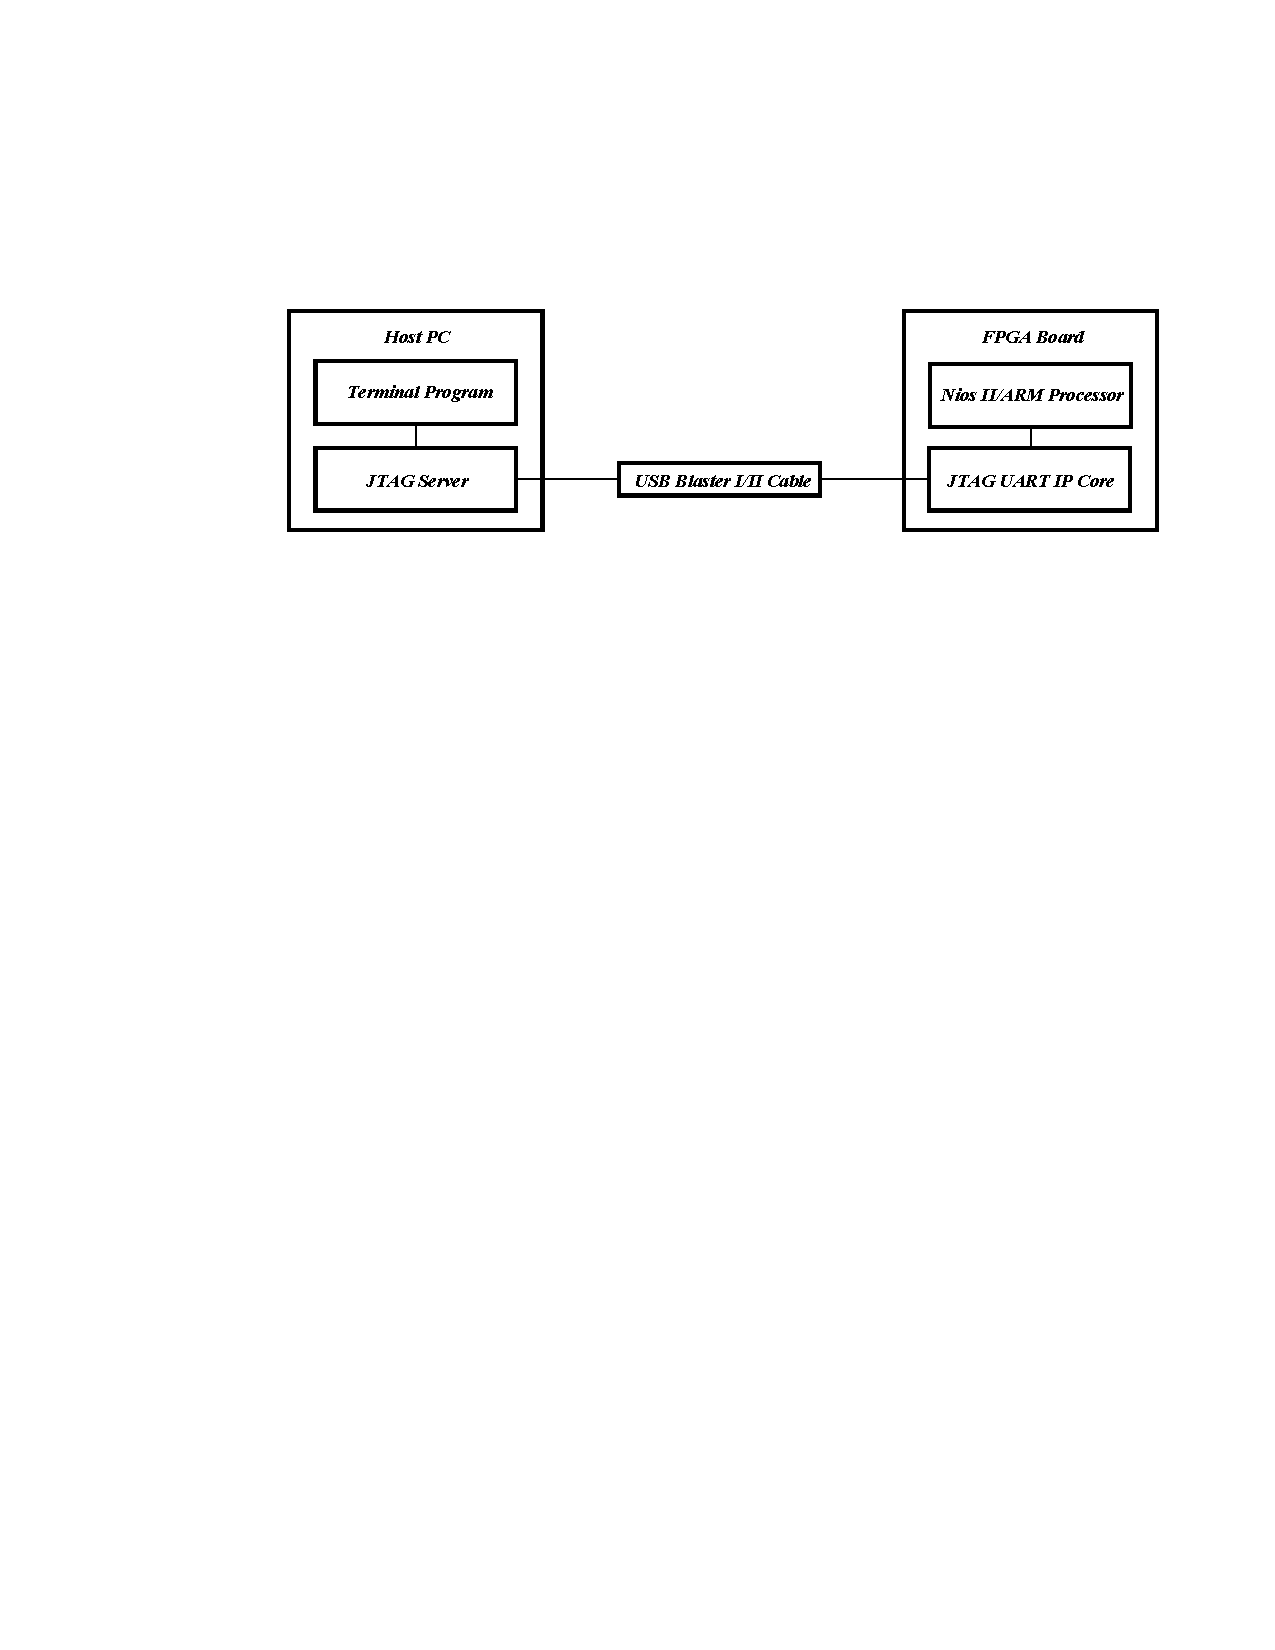
\includegraphics{figures/fig_jtag_uart_communication_link.pdf}
   \end{center}
   \caption{A JTAG UART communication link between the host PC and the FPGA board.}
	\label{fig:jtag_uart_communication_link}
\end{figure}

\subsubsection{Using the JTAG UART Register Interface}

The JTAG UART includes a transmit (TX) FIFO queue that stores data 
waiting to be transmitted to the host computer. The size of this FIFO queue is 64 characters by default, and can be configured when the core is instantiated in Platform Designer.  
Character data is loaded into this FIFO queue by performing a write to bits 7$-$0
of the {\it Data} register in Figure \ref{fig:jtag_uart_regmap}.  
Note that writing into this register has no effect 
on received data.  The amount of space, {\it WSPACE}, currently available in the TX FIFO queue is 
provided in bits 31$-$16 of the {\it Control} register.  If
the TX FIFO queue is full, then any characters written to the {\it Data} register will be lost.

\begin{figure}[h!]
   \begin{center}
       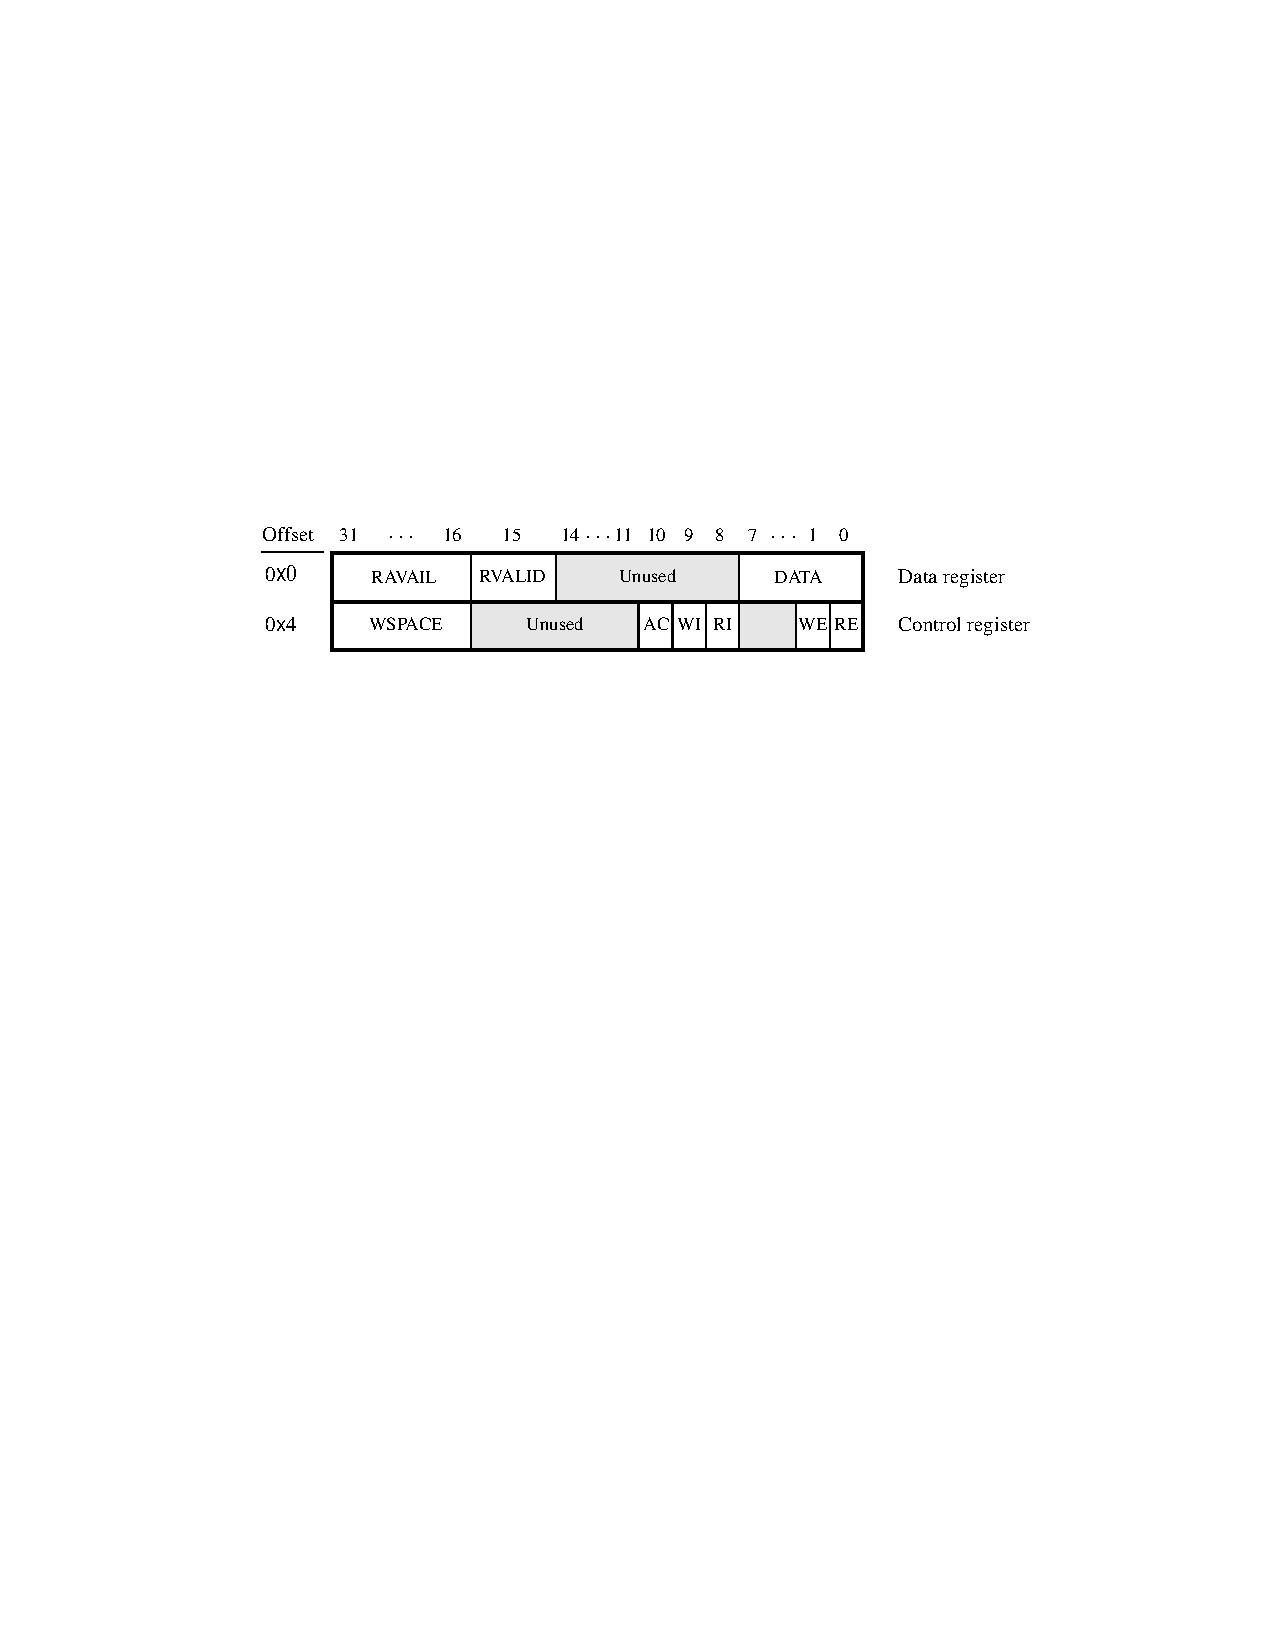
\includegraphics{figures/fig_jtaguart_regmap.pdf}
   \end{center}
   \caption{JTAG UART registers.}
	\label{fig:jtag_uart_regmap}
\end{figure}

When character data from the host computer is received by the JTAG UART 
it is stored in a receive (RX) FIFO queue. The size of this FIFO queue is 64 characters by default, and can be configured when the core is instantiated in Platform Designer. The number of characters currently stored in this FIFO queue is
indicated in the field {\it RAVAIL}, which are
bits 31$-$16 of the {\it Data} register.  If the RX FIFO queue overflows, then
additional data is lost. When data is present in the RX FIFO queue, then the value of {\it RAVAIL} will be 
greater than 0 and the value of bit 15, {\it RVALID}, will be 1. Reading the character at
the head of the FIFO queue, which is provided in bits $7-0$, decrements the value of {\it RAVAIL} 
by one and returns this decremented value as part of the read
operation. If no data is present in the RX FIFO queue, then {\it RVALID} will 
be set to 0 and the data in bits $7-0$ is invalid.

Bit 10 in the {\it Control} register, called {\it AC}, has the value 1 if the JTAG UART has been
accessed by the host computer. This bit can be used to check if a working connection to
the host computer has been established. The {\it AC} bit can be cleared to 0 by writing a 1
into it. 

The {\it WE} and {\it RE} bits of the {\it Control} register can be set to 1 to enable write and read interrupts, respectively. The {\it WI} and {\it RI} bits have the value 1 if a write or read interrupt is pending, respectively. This tutorial does not describe the use of interrupts with the JTAG UART IP Core.

\subsubsection{Using the JTAG* UART with C Code}

Figure \ref{fig:jtag_uart_c} shows two C functions for reading and writing the JTAG UART, respectively. 
The \textit{get\_char} function attempts to read a previously unread character from the JTAG UART, and returns that character if successful. If a previously unread character is not available in the RX FIFO queue a null character `$\backslash$0' is returned instead. 

The \textit{put\_char} function attempts to write a character to the JTAG UART. It succeeds if there is space available in the TX FIFO queue of the JTAG UART which it determines by reading bits 31$-$16 of the \textit{Control} register. If there is no space, the function does not write the character to the JTAG UART.

An example C program that demonstrates the use of the JTAG UART is made available as part of the  
\productNameMed{}. The example can be found under the heading {\it sample programs}, 
and is identified by the name {\it JTAG UART}.

\begin{figure}[h!]
\lstinputlisting[language=C]{design_files/jtag_uart.c}
\caption{C-language functions that use the JTAG UART.}
   \label{fig:jtag_uart_c}
\end{figure}

\subsubsection{Using the JTAG* UART with Nios\textsuperscript{\textregistered} II Assembly Code}

Figure \ref{fig:jtag_uart_nios} shows two Nios II assembly-language subroutines for reading and writing the JTAG UART. 
The \textit{GET\_CHAR} subroutine reads a character from the JTAG UART, and returns that character in register r2. If the JTAG UART's RX FIFO queue is empty, it returns the null character `$\backslash$0'. 

The \textit{PUT\_CHAR} subroutine attempts to write a character to the JTAG UART. It succeeds if there is space available in the TX FIFO queue of the JTAG UART which it determines by reading bits 31$-$16 of the \textit{Control register}. If there is no space, the subroutine skips the \textit{stwio} instruction, thus not writing the character to the JTAG UART.

An example Nios II assembly-language program that demonstrates the use of the JTAG UART is made available as part of the  
\productNameMed{}. The example can be found under the heading {\it sample programs}, 
and is identified by the name {\it JTAG UART}.

\begin{figure}[h!]
\lstinputlisting[style=defaultNiosStyle]{design_files/jtag_uart_nios.s}
\caption{Nios II assembly-language subroutines that use the JTAG
UART.}
   \label{fig:jtag_uart_nios}
\end{figure}
\pagebreak
\clearpage
\newpage


\subsubsection{Using the JTAG* UART with ARM Assembly Code}

Figure \ref{fig:jtag_uart_arm} shows two ARM assembly-language subroutines for reading and writing the JTAG UART, respectively. 
The \textit{GET\_CHAR} subroutine reads a character from the JTAG UART, and returns that character in register R0. If the JTAG UART's RX FIFO queue is empty, it returns the null character `$\backslash$0'.

The \textit{PUT\_CHAR} subroutine attempts to write a character to the JTAG UART. It succeeds if there is space available in the TX FIFO queue of the JTAG UART which it determines by reading bits 31$-$16 of the \textit{Control} register. If there is no space, the subroutine skips the \textit{STR} instruction, thus not writing the character to the JTAG UART.

An example ARM assembly-language program that demonstrates the use of the JTAG UART is made available as part of the  
\productNameMed{}. The example can be found under the heading {\it sample programs}, 
and is identified by the name {\it JTAG UART}.

\begin{figure}[h!]
\lstinputlisting[style=defaultArmStyle]{design_files/jtag_uart_arm.s}
\caption{ARM assembly-language subroutines that use the JTAG
UART.}
   \label{fig:jtag_uart_arm}
\end{figure}
\pagebreak
\clearpage
\newpage

%\subsubsection{Connecting to the JTAG UART from the Host PC Using Altera Monitor Program}

\subsection{The RS232 UART Terminal}

The RS232 UART is an IP core that facilitates serial UART communication between the system on the FPGA board and the host PC, through an RS232 cable. Figure \ref{fig:rs232_uart_communication_link} shows the arrangement of the components used to facilitate this communication link.  While this serial communication link can be used to transmit any arbitrary data, it is in practice commonly used to transmit character data. On the FPGA board, a program running on the Nios II or ARM processor can use the RS232 core's memory-mapped register interface shown in Figure \ref{fig:rs232_uart_regmap} to send and receive character data to and from the host PC.

\begin{figure}[h!]
   \begin{center}
       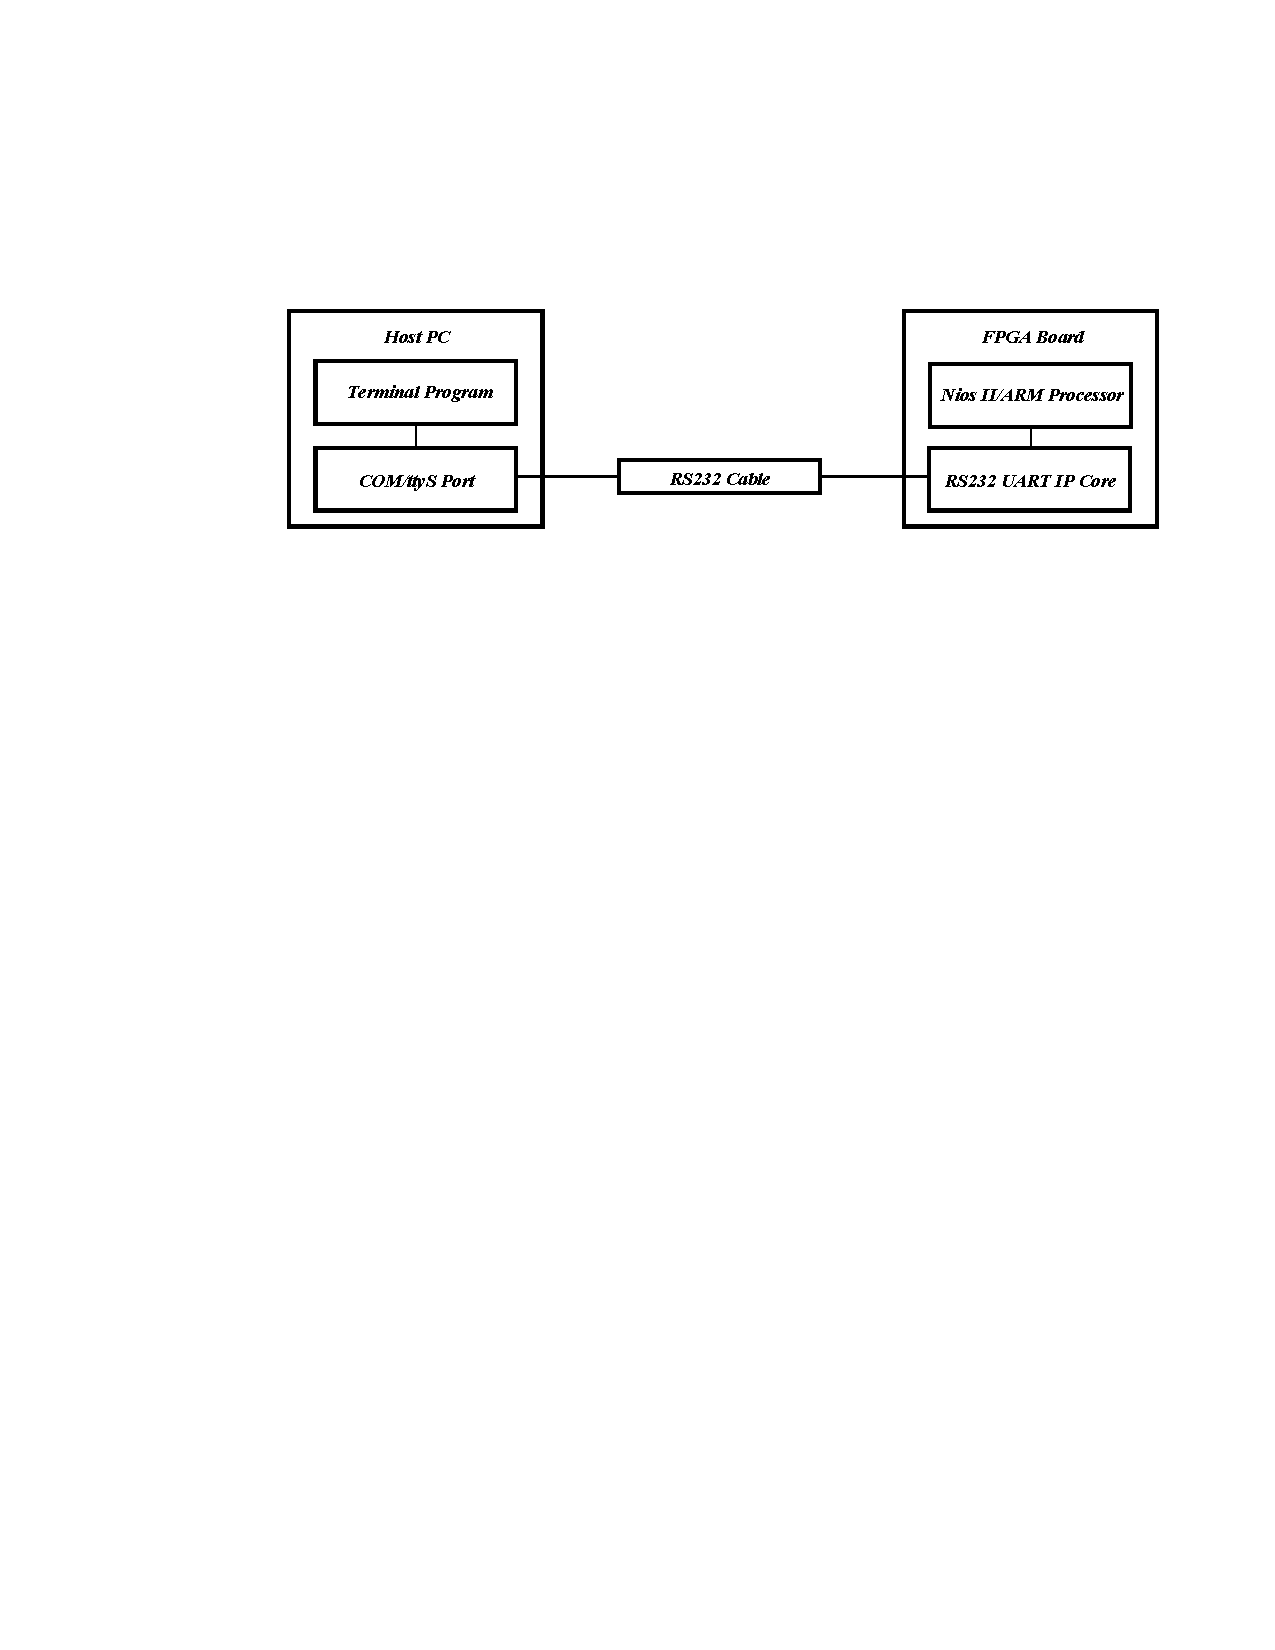
\includegraphics[scale=1.0]{figures/fig_rs232_uart_communication_link.pdf}
   \end{center}
   \caption{An RS232 UART communication link between the host PC and the FPGA board.}
	\label{fig:rs232_uart_communication_link}
\end{figure}

When the RS232 UART is connected to a host PC via an RS232 cable, the PC will recognize it as a serial communication device. On a Windows\textsuperscript{\textregistered} PC, it will appear as a \textit{COM} port (in \textit{Device Manager}). On a Linux PC, it will appear as a \textit{ttyS} character device (in \textit{/dev/}). There exist many terminal programs that can be used to communicate with a serial communication device, and documentation for them can be found online. Section \ref{sec:putty_uart} of this tutorial demonstrates the use of a popular and free terminal called \textit{Putty} to communicate with the RS232 UART.

\subsubsection{Using the RS232 UART Register Interface}
\label{sec:rs232_reg}

\begin{figure}[h!]
   \begin{center}
       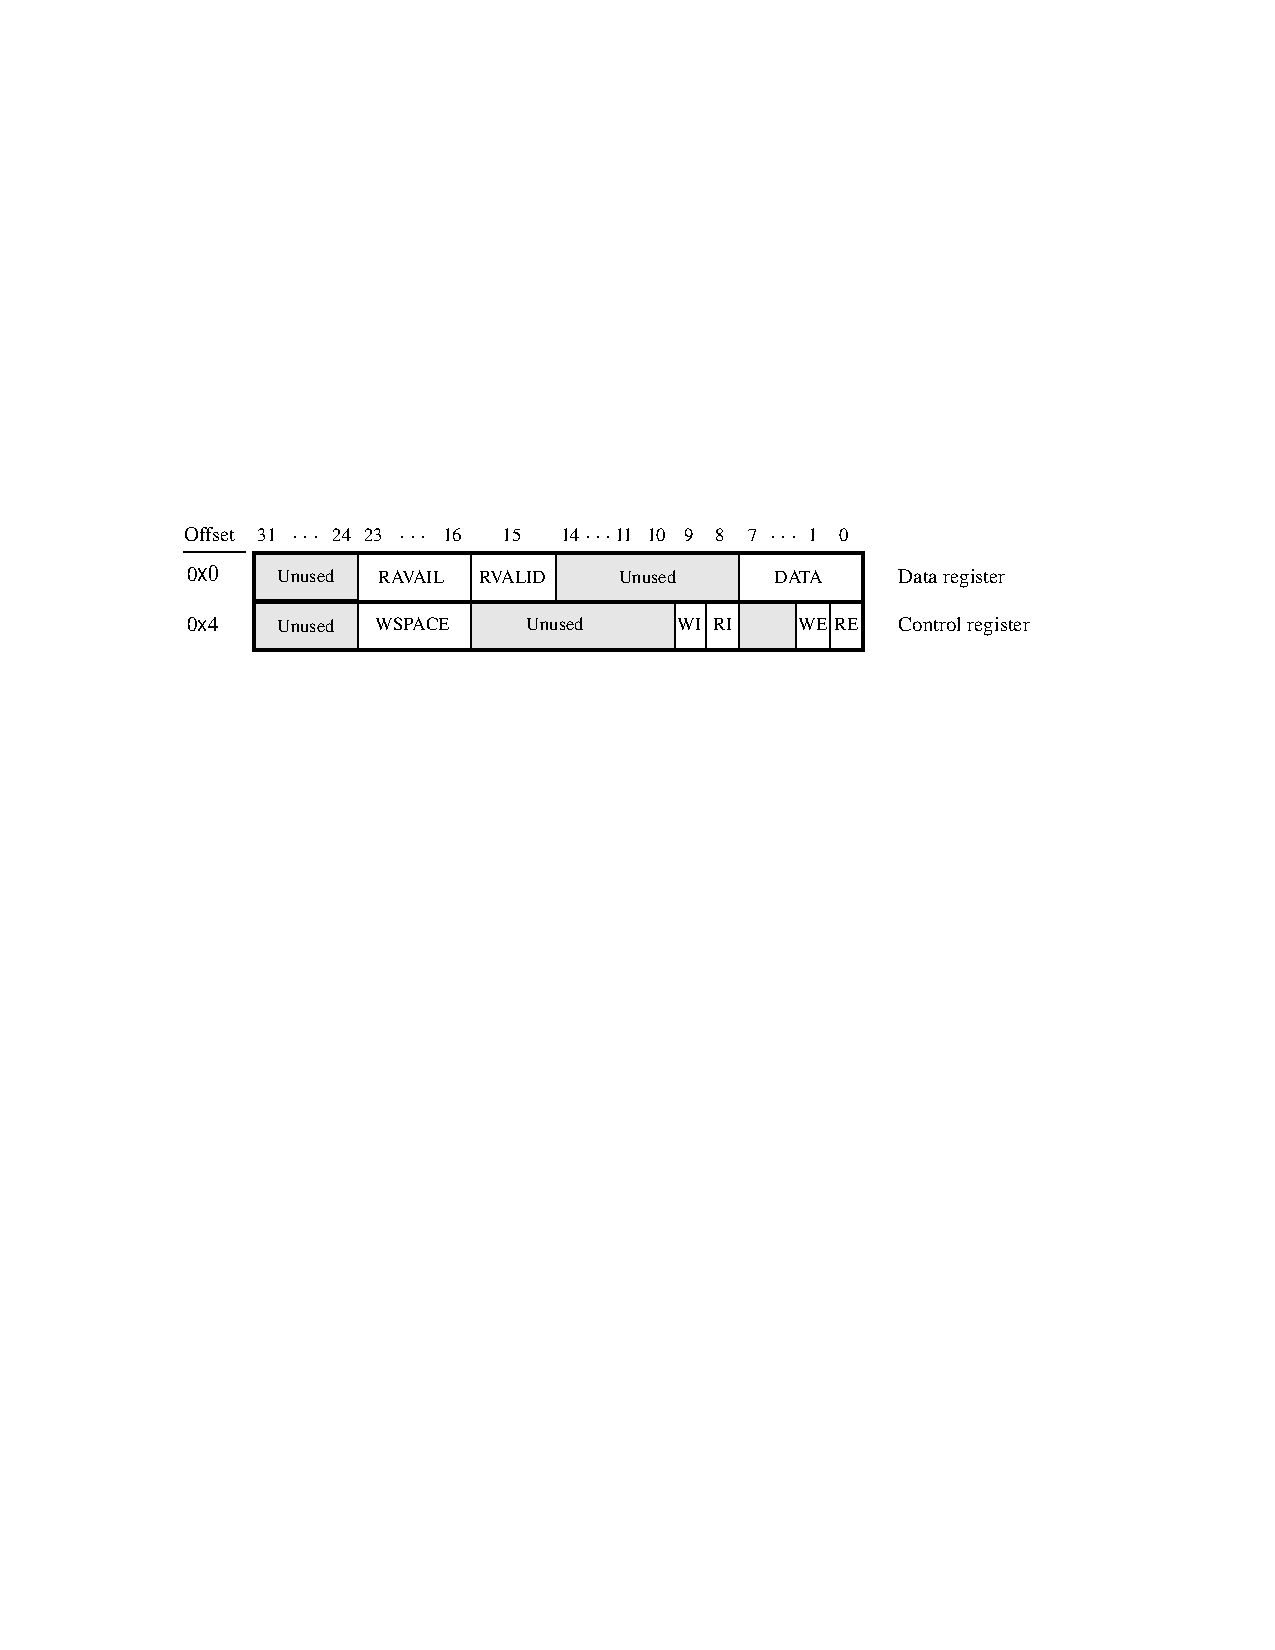
\includegraphics{figures/fig_rs232uart_regmap.pdf}
   \end{center}
   \caption{RS232 UART registers.}
	\label{fig:rs232_uart_regmap}
\end{figure}

The RS232 UART includes a transmit (TX) FIFO queue that stores data 
waiting to be transmitted to the host computer. Character data is loaded into this FIFO queue by performing a write to bits 7$-$0
of the {\it Data} register in Figure \ref{fig:rs232_uart_regmap}.  
Note that writing into this register has no effect 
on received data.  The amount of space, {\it WSPACE}, currently available in the TX FIFO queue is 
provided in bits 23$-$16 of the {\it Control} register.  If
the TX FIFO queue is full, then any characters written to the {\it Data} register will be lost.

When character data from the host computer is received by the RS232 UART 
it is stored in a receive (RX) FIFO queue. The number of characters currently stored in this FIFO queue is
indicated in the field {\it RAVAIL}, which are
bits 23$-$16 of the {\it Data} register.  If the RX FIFO queue overflows, then
additional
data is lost. When data is present in the RX FIFO queue, then the value of {\it RAVAIL} will be 
greater than 0 and the value of bit 15, {\it RVALID}, will be 1. Reading the character at
the head of the FIFO queue, which is provided in bits $7-0$, decrements the value of {\it RAVAIL} 
by one and returns this decremented value as part of the read
operation. If no data is present in the RX FIFO queue, then {\it RVALID} will 
be set to 0 and the data in bits $7-0$ is invalid.

The {\it WE} and {\it RE} bits of the {\it Control} register can be set to 1 to enable write and read interrupts, respectively. The {\it WI} and {\it RI} bits have the value 1 if a write or read interrupt is pending, respectively.  This tutorial does not describe the use of interrupts with the RS232 UART IP Core.

\subsubsection{Using the RS232 UART with C Code}
\label{sec:rs232_c}

Figure \ref{fig:rs232_uart_c} shows two C functions for reading and writing the RS232 UART, respectively. 
The \textit{get\_char} function attempts to read a previously unread character from the RS232 UART, and returns that character if successful. If a previously unread character is not available in the RX FIFO queue a null character `$\backslash$0' is returned instead. 

The \textit{put\_char} function attempts to write a character to the RS232 UART. It succeeds if there is space available in the TX FIFO queue of the RS232 UART which it determines by reading bits 23$-$16 of the \textit{Control} register. If there is no space, the function does not write the character to the RS232 UART.

\begin{figure}[h!]
\lstinputlisting[language=C]{design_files/rs232.c}
\caption{C-language functions that use the RS232 UART.}
   \label{fig:rs232_uart_c}
\end{figure}

\subsubsection{Using the RS232 UART with Nios\textsuperscript{\textregistered} II Assembly Code}
\label{sec:rs232_nios}

Figure \ref{fig:rs232_uart_nios} shows two Nios II assembly-language subroutines for reading and writing the RS232 UART, respectively. 
The \textit{GET\_CHAR} subroutine reads a character from the RS232 UART, and returns that character in register r2. If the RS232 UART's RX FIFO queue is empty, it returns the null character `$\backslash$0'. 

The \textit{PUT\_CHAR} subroutine attempts to write a character to the RS232 UART. It succeeds if there is space available in the TX FIFO queue of the RS232 UART which it determines by reading bits 23$-$16 of the \textit{Control register}. If there is no space, the subroutine skips the \textit{stwio} instruction, thus not writing the character to the RS232 UART.

\begin{figure}[h!]
\lstinputlisting[style=defaultNiosStyle]{design_files/rs232_nios.s}
\caption{Nios II assembly-language subroutines that use the RS232
UART.}
   \label{fig:rs232_uart_nios}
\end{figure}
\pagebreak
\clearpage
\newpage


\subsubsection{Using the RS232 UART with ARM\textsuperscript{\textregistered} Assembly Code}
\label{sec:rs232_arm}

Figure \ref{fig:rs232_uart_arm} shows two ARM assembly code subroutines for reading and writing the RS232 UART, respectively. 
The \textit{GET\_CHAR} subroutine reads a character from the RS232 UART, and returns that character in register R0. If the RS232 UART's RX FIFO queue is empty, it returns the null character `$\backslash$0'.

The \textit{PUT\_CHAR} subroutine attempts to write a character to the RS232 UART. It succeeds if there is space available in the TX FIFO queue of the RS232 UART which it determines by reading bits 23$-$16 of the \textit{Control register}. If there is no space, the subroutine skips the \textit{STR} instruction, thus not writing the character to the RS232 UART.

\begin{figure}[h!]
\lstinputlisting[style=defaultArmStyle]{design_files/rs232_arm.s}
\caption{ARM assembly language subroutines that use the RS232
UART.}
   \label{fig:rs232_uart_arm}
\end{figure}
\pagebreak
\clearpage
\newpage

\subsubsection{Connecting to the RS232 UART from the Host PC Using Putty}
\label{sec:putty_uart}

Putty is a popular free-to-use terminal program that can be used to communicate with serial character devices attached to the PC. This section describes how to use Putty to connect to the RS232 UART on a Windows host PC. 

On a Windows PC, serial communication devices such as the RS232 UART are recognized by the PC as COM ports. As there can be multiple COM ports connected to the PC, each COM port is assigned a unique identifying number. The number assigned to the RS232 UART can be determined by viewing the list of COM ports in \textit{Device Manager}. Figure \ref{fig:putty_0} shows the \textit{Device Manager's} list of available COM ports on one particular PC. Here, there was only one COM port (the RS232 UART) connected which had been assigned the number 5 (COM5). In the case where there are many COM ports available, the number assigned to the RS232 UART can be determined by disconnecting and reconnecting the cable to see which COM port disappears then reappears in the list.

\begin{figure}[h!]
   \begin{center}
       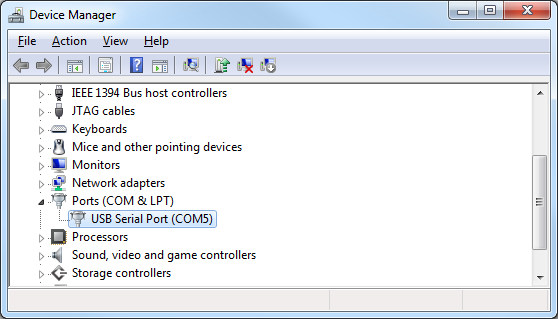
\includegraphics[scale=0.7]{figures/fig_putty_tut_0}
   \end{center}
   \caption{Determining the COM number assigned to the RS232 UART in Device Manager.}
	\label{fig:putty_0}
\end{figure}

Once the COM port corresponding to the RS232 UART is determined, Putty can be configured to connect to it. Figure \ref{fig:putty_1} shows the main window of Putty. In this window, the \textit{Serial} connection type must be chosen, and the COM port must be entered in the  \textit{Serial line} field, as shown in the figure. 

\begin{figure}[h!]
   \begin{center}
       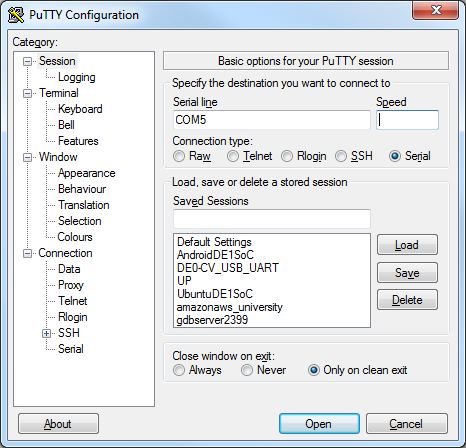
\includegraphics[scale=0.7]{figures/fig_putty_tut_1}
   \end{center}
   \caption{Putty's main window.}
	\label{fig:putty_1}
\end{figure}

\begin{figure}[h!]
   \begin{center}
       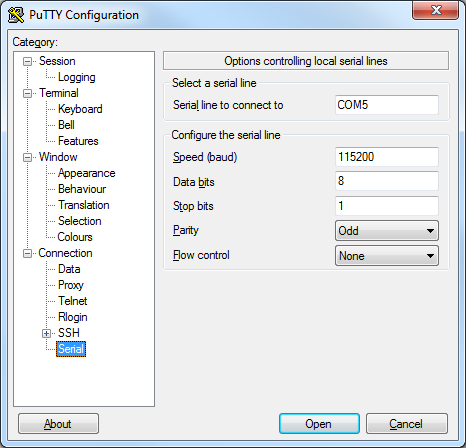
\includegraphics[scale=0.8]{figures/fig_putty_tut_2}
   \end{center}
   \caption{Putty's configuration window for serial communication settings.}
	\label{fig:putty_2}
\end{figure}

Some additional details about the RS232 UART must be entered by selecting the \textit{Serial} panel in the \textit{Category} box on the left side of the window. The \textit{Serial} panel is shown in Figure \ref{fig:putty_2}. These settings must be configured to match the settings that were chosen when instantiating the RS232 UART IP core. Figure \ref{fig:putty_3} shows the parameters that are set when instantiating the core in \textit{Platform Designer}, including the \textit{Baud rate}, \textit{Parity}, \textit{Data bits}, and \textit{Stop bits}. The \textit{Flow control} option should be set to \textit{None} as the RS232 UART IP core does not support any flow control protocol.

The \textit{Speed} option refers to the \textit{baud rate} of the the RS232 UART, which is the number of bits per second that the RS232 UART will send, and is expecting to receive from the host PC. The \textit{Data bits} option refers to how many bits of data will be transmitted in each packet. Eight data bits are typically used for transmitting ASCII characters. The \textit{Stop bits} refer to how many bits follow the data bits to indicate that the packet is ending. The \textit{Parity} option refers to the error-checking scheme to use to determine if there is data corruption in incoming packets. The \textit{Flow control} option refers to the handshaking protocol by which either end of the connection can request to pause and resume transmission of data. 

\begin{figure}[h!]
   \begin{center}
       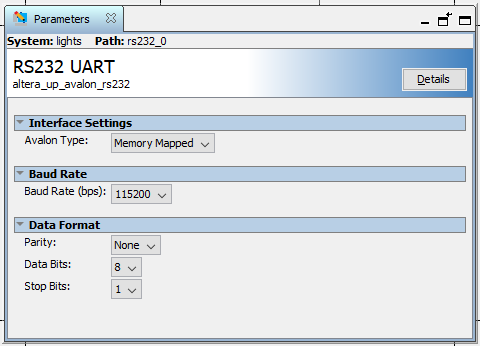
\includegraphics[scale=0.7]{figures/fig_putty_tut_3}
   \end{center}
   \caption{RS232 UART settings in Platform Designer Wizard.}
	\label{fig:putty_3}
\end{figure}

Once all of the serial line settings have been entered, the \textit{Open} button can be pressed to start the terminal. Once opened, a terminal will appear as shown in Figure \ref{fig:putty_4}. This terminal will now display text coming from the RS232 UART, and send any user inputs to the RS232 UART.

\begin{figure}[h!]
   \begin{center}
       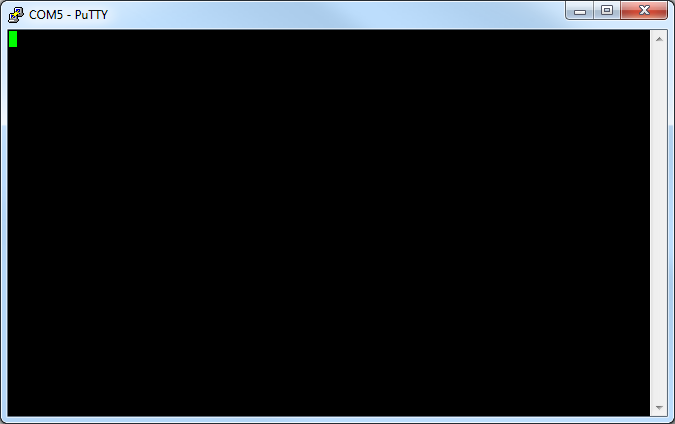
\includegraphics[scale=0.7]{figures/fig_putty_tut_4}
   \end{center}
   \caption{Putty terminal ready to communicate with RS232 UART.}
	\label{fig:putty_4}
\end{figure}

\subsection{The USB UART Terminal}

Serial UART communication to facilitate terminal communication in the past was commonly done using an RS232 cable. As modern computers have adopted the USB cable as the preferred connection medium, few computers now have RS232 ports. As a result, USB-to-UART chips are often used to allow systems (such as a system on a DE-series board) to perform serial UART communication over USB cable with a host PC. The DE1-SoC board contains the \textit{FTDI FT232R} USB-to-UART chip and is capable of this communication link. Figure \ref{fig:usb_uart_communication_link} shows the arrangement of the components that are used to facilitate this communication link.

On the FPGA board, the USB-to-UART chip exposes an RS232 interface, which comprises an RX (receive) pin, and a TX (transmit) pin. The RS232 UART IP core can be instantiated to communicate through these pins. A program running on a Nios II or ARM processor on the board can then use this IP core's register interface, described in section \ref{sec:rs232_reg}, to send and receive characters to the host PC. C code that uses this interface is shown in section \ref{sec:rs232_c}. Nios II assembly-language code that uses this interface is shown in section \ref{sec:rs232_nios}. ARM assembly-language code that uses this interface is shown in section \ref{sec:rs232_arm}.

\begin{figure}[h!]
   \begin{center}
       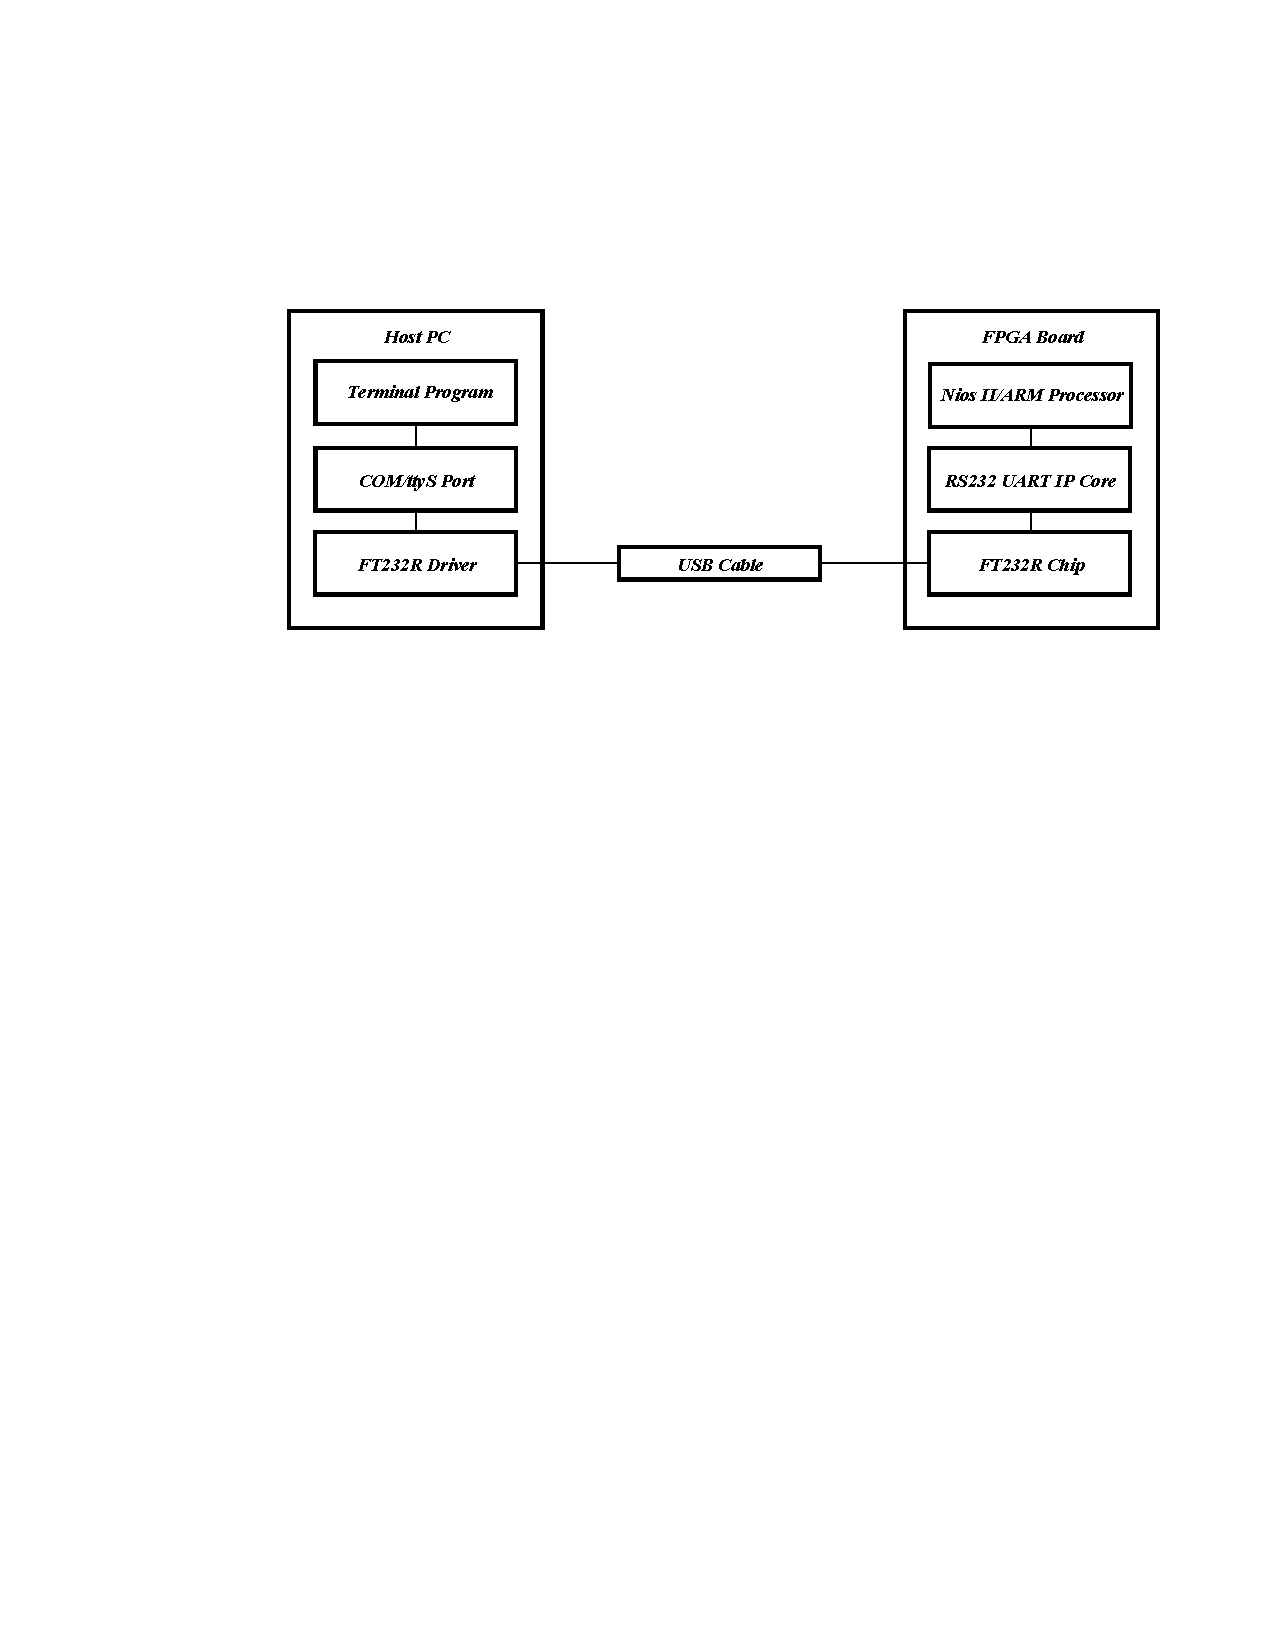
\includegraphics[scale=1.0]{figures/fig_usb_uart_communication_link.pdf}
   \end{center}
   \caption{A USB UART communication link between the host PC and the FPGA board.}
	\label{fig:usb_uart_communication_link}
\end{figure}

On the host PC side, the driver for the \textit{FTDI FT232R} chip detects that the chip is connected via a USB cable, and exposes it as a serial communication device. On a Windows PC, it will appear as a \textit{COM} port (in \textit{Device Manager}). On a Linux PC, it will appear as a \textit{ttyS} character device (in \textit{/dev/}). A terminal program can connect to the exposed COM/ttyS interface to send and receive characters with the system on the FPGA board. There exist many terminal programs that can be used, and documentation for them can be found online. Section \ref{sec:putty_uart} of this tutorial demonstrates the use of a popular and free terminal program called \textit{Putty}.

\subsection{The ARM Semihosting Terminal}

%When a debugger such as the Altera Monitor Program starts a debugging session with a CPU, it establishes a communication link to the processor. It is through this link that the debugger performs operations such as single-stepping and setting breakpoints. Semihosting is a mechanism that leverages this connection to allow a program running on an ARM processor to request services from the debugger. Among other possible services, a program can request to read and write special files \textit{stdin} and \textit{stdout}. These files and are not stored in any persistent storage device. Rather, they are temporary buffers that are allocated inside the Altera Monitor Program. When a program writes characters to the \textit{stdout} file, the Altera Monitor Program displays those characters in its Semihosting Terminal. When a user enters characters to the Semihosting Terminal, these characters are stored in the \textit{stdin} buffer and are sent to the program when it reads the \textit{stdin} file.

When a debugger such as the \productNameMed{} starts a debugging session with a processor, it establishes a communication link to the processor. It is through this link that the debugger performs operations such as single-stepping and setting breakpoints. Semihosting is a mechanism that leverages this connection to allow a program running on an ARM processor to request services from the debugger. Among other possible services, a program can request to read and write files. When a program writes characters to a special file named \textit{stdout}, the \productNameMed{} displays those characters in its Semihosting terminal. When a user enters characters to the Semihosting terminal, these characters are stored in a special file named \textit{stdin} which can be read by the program. Note that \textit{stdout} and \textit{stdin} are not actually files, and are not stored in persistent storage. They are temporary buffers allocated inside the \productNameMed{}, and are lost when the \productNameMed{} closes.

To use the Semihosting Terminal in the \productNameMed{}, users must select it under the \textit{Terminal device} drop-down menu in the \textit{System Settings} window. Once selected, the \productNameMed{}'s \textit{Terminal window} will function as a Semihosting terminal upon starting a debugging session with the ARM processor.

The following subsection describes how to write ARM programs in C to use the Semihosting interface to read and write \textit{stdin} and \textit{stdout}. It is not recommended to use the Semihosting interface in assembly-language code. When writing ARM assembly-language programs, the JTAG UART or RS232 UART should be used instead.

\subsubsection{Using Semihosting with C Code}

The ARM C compiler that is used in the \productNameMed{} uses special C libraries that have been modified to use the Semihosting interface. Standard I/O functions such as printf, scanf, puts, and fprintf that are built into these libraries will automatically use Semihosting services to perform their respective tasks. This provides a Linux-like way to perform terminal communication, with no need to manually interface with the underlying communication link. Figure \ref{fig:semihosting_c} shows an example C program that uses these functions to print strings to the terminal and accept input from the user. 

\begin{figure}[h!]
\lstinputlisting[language=C]{design_files/semihosting.c}
\caption{ARM C code that uses the Semihosting terminal.}
   \label{fig:semihosting_c}
\end{figure}

%\subsubsection{Using Semihosting with ARM Assembly Code}

%To request a Semihosting operation, a program running on the ARM processor calls the SVC (supervisor call) instruction with a special argument "0x123456". Doing this will cause a SVC exception, and execution will jump to the SVC exception vector. At this point, if there is a Semihosting-capable debugger connected to the CPU, the CPU will halt execution. The debugger will then read the arguments passed to the operation (which the program placed in R0 and R1 prior to calling SVC) to determine what Semihosting service is being requested, and with what data. The debugger then performs the requested service and returns any requested data in R0 and/or a buffer in memory.

%SVC 0x123456 is by convention understood to be a Semihosting call. 

%In the case of the Altera Monintor Program, a breakpoint is placed at the SVC exception vector to facilitate the halting. Once halted, the Altera Monitor Program checks if 

%While it is possible to invoke these semihosting calls manually, it is discouraged. When running an ARM assembly program, without the ability to call stdio library functions, it is highly recommended to use another Terminal such as the JTAG UART Terminal.

%The ARM Semihosting terminal is unlike the other terminals mentioned in this tutorial in that it does not use the UART protocol at any point in the FPGA board to host PC communication link. Instead, the ARM Semihosting terminal sends and receives character data to and from the FPGA board through the JTAG debugging connection made by the Altera Monitor Program. 

\section{Conclusion}

This tutorial demonstrated the use of the different terminals available for communicating with programs running on DE-series boards. 

% Copyright and Trademark

%\newcommand{\datePublished}{Mar 2022}

\newcommand{\versnum}{21.1} %version number quartus/AMP
\newcommand{\quartusname}{Quartus\textsuperscript{\textregistered} Prime}	
\newcommand{\textBar}{For \quartusname{} \versnum{}}
\newcommand{\thisyear}{2022 } %for copyright
\newcommand{\company}{FPGAcademy.org}
\newcommand{\longteamname}{FPGAcademy.org}
\newcommand{\teamname}{FPGAcademy}
\newcommand{\website}{FPGAcademy.org}

\newcommand{\productAcronym}{AMP}
\newcommand{\productNameShort}{Monitor Program}

\newcommand{\productNameMedTM}{Monitor Program}
\newcommand{\productNameMed}{Monitor Program}

%\newcommand{\headerLogoFilePath}[1]{#1/FPGAcademy.png}



%%%%%%%%%%%%%%%%%%%%%%%%%%%%%%%%%%%%%%%%
%%% FPGAcademy Copyright Information %%%
%%%%%%%%%%%%%%%%%%%%%%%%%%%%%%%%%%%%%%%%

%Always put the copyright on a new page (clear page), with some vertical space from top
\clearpage
\vspace{1in}

\noindent

Copyright {\copyright} FPGAcademy.org. All rights reserved. FPGAcademy and the FPGAcademy logo are trademarks of  FPGAcademy.org.  This document is being provided on an ``as-is'' basis and as an accommodation and therefore all warranties, representations or guarantees of any kind (whether express, implied or statutory) including, without limitation, warranties of merchantability, non-infringement, or fitness for a particular purpose, are specifically disclaimed.

%FPGAcademy assumes no responsibility or liability arising out of the application or use of any information,  product,  or  service  described  herein  except  as  expressly  agreed  to  in  writing  by  FPGAcademy.



**Other names and brands may be claimed as the property of others.



\end{document}
